\documentclass[11pt]{beamer}
\usetheme{Warsaw}
\usepackage[utf8]{inputenc}
\usepackage[german]{babel}
\usepackage[T1]{fontenc}
\usepackage{amsmath}
\usepackage{amsfonts}
\usepackage{amssymb}
\usepackage{graphicx}
\author{Erik Zimmermann}
\title{Gedämpfter LC Schwingkreis Oszilloskop, Teilversuch 4.4.1}
%\setbeamercovered{transparent} 
%\setbeamertemplate{navigation symbols}{} 
%\logo{} 
%\institute{} 
%\date{} 
%\subject{} 
\begin{document}

\begin{frame}
\titlepage
\end{frame}

%\begin{frame}
%\tableofcontents
%\end{frame}

\begin{frame}{Versuchsaufbau und Durchführung}
\begin{figure}[H]
\centering
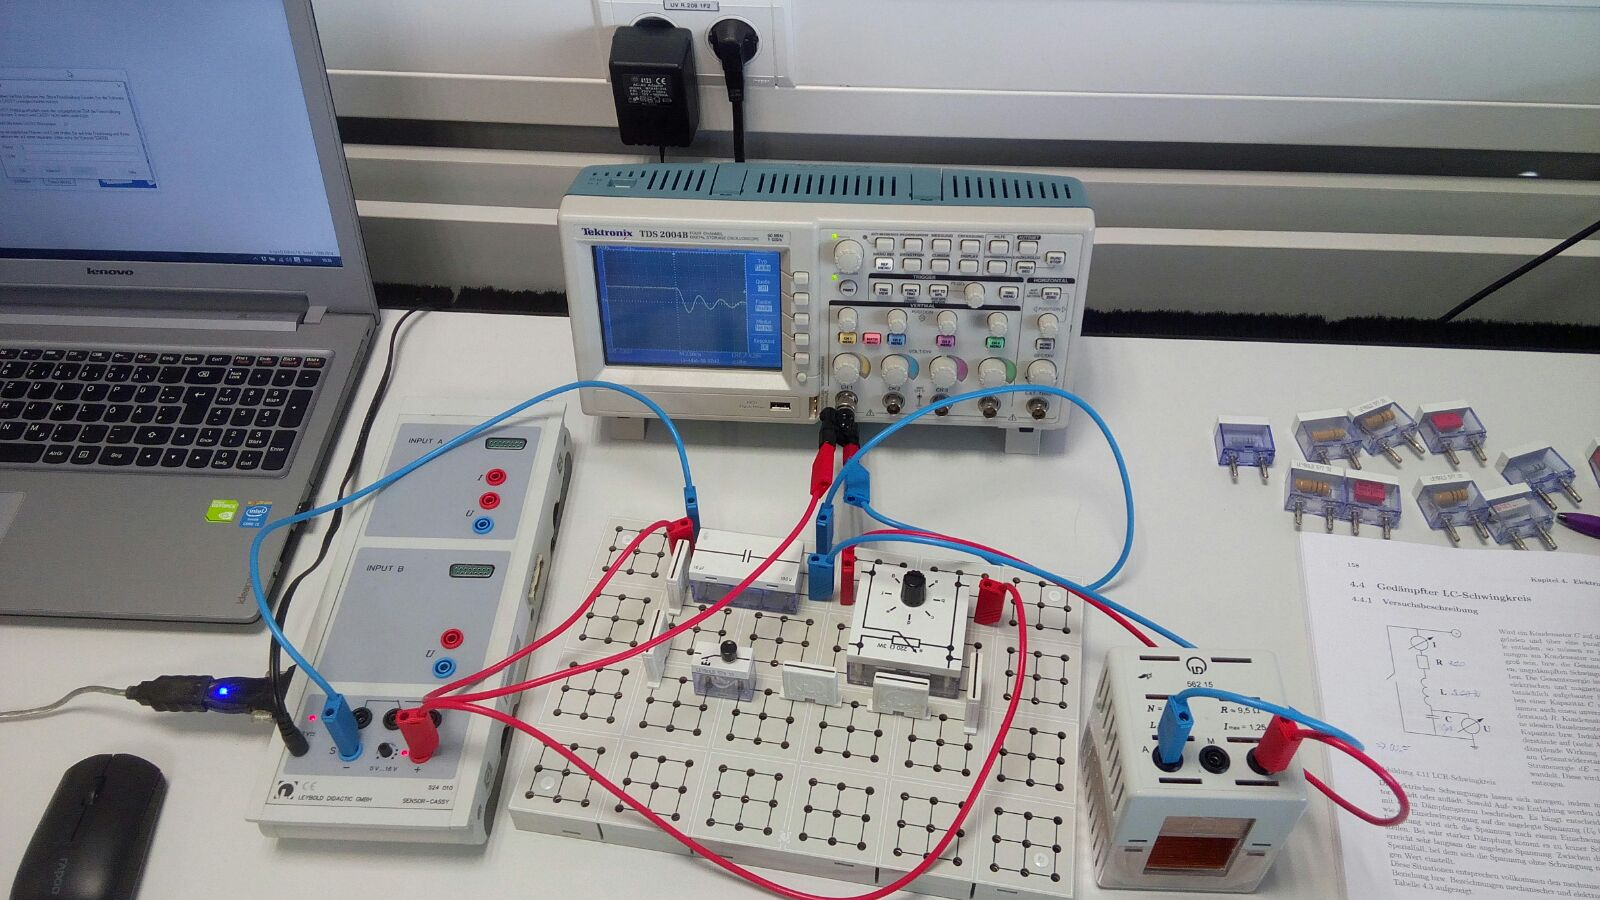
\includegraphics[scale=0.20]{ArbeitsplatzE_1.jpg}
\caption{Versuchsaufbau}
\end{figure}
\end{frame}

\begin{frame}
\begin{itemize}
\item Alle Versuche wurden bei einer Eingangspannung von $U_0=5.6V$ durchgeführt, dabei wurde das Oszilloskop auf \glqq Single Sequence\grqq $\,$ eingestellt.
\item Aus dem resultierenden Standbild wurden die Spannungsmaxima mit entsprechenden Zeitwerten abgelesen.
\item Die Ablesefehler wurden zu $\sigma_U=\frac{0.08}{\sqrt{12}}V$ \& $\sigma_T=\frac{100\cdot 10^{-6}}{\sqrt{12}}s$ bestimmt.
\end{itemize}
\end{frame}

\begin{frame}{Rohdaten (beispielhaft)}
\begin{table}[H]\centering
\caption{1. Messung}
\begin{tabular}{c|c}
\hline
$U_1=3.12V$& $t_1=0.5ms$\\ 
$U_2=1.76V$& $t_2=4.4ms$\\ 
$U_3=1.04V$& $t_3=8.2ms$ \\
$U_4=0.56V$& $t_4=12.0ms$ \\
\end{tabular} 
\end{table}
\begin{figure}[H]\centering
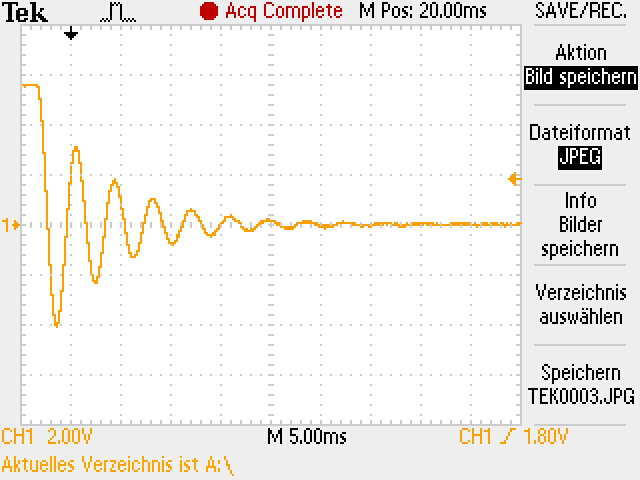
\includegraphics[scale=0.7]{TEK0003.JPG}
\caption{Beispiel: Messung 1}
\end{figure}
\end{frame}

\begin{frame}{Transformation der Rohdaten}
\begin{table}[H]\centering
\caption{Messung 1}
\begin{tabular}{c|c|c|c}
Frequenz in Hz & $\sigma_f$ in Hz & Abklingkoeffizient in $\frac{1}{s}$ & $\sigma_{\delta}$ in $\frac{1}{s}$\\ 
\hline
$f=256.410$& $\sigma_f=1.898$& $\delta=150.047$& $\sigma_{\delta}=4.264$\\ 
$f=263.158$& $\sigma_f=1.999$& $\delta=143.827$& $\sigma_{\delta}=7.260$\\
$f=263.158$& $\sigma_f=1.999$& $\delta=174.551$& $\sigma_{\delta}=13.535$\\
\end{tabular} 
\end{table}

Hier wurden die Fehler aus den folgenden Gleichungen ermittelt:
\begin{align}
\sigma_f&=\frac{\sigma_T}{T^2}\\
\sigma_{\delta_n}&=\frac{1}{T_n}\cdot \sqrt{(\frac{\sigma_{U_n}}{U_n})^2+(\frac{\sigma_{U_{n+1}}}{U_{n+1}})^2+(\delta_n\cdot \sigma_{T_n})^2}
\end{align}
Der Abklingkoeffizient $\delta$ wird bestimmt aus:
\begin{align}
\delta_n&=\frac{\ln{\frac{U_n}{U_{n+1}}}}{t_{n+1}-t_n}
\end{align}
\end{frame}

\begin{frame}{Ergebnis}
Aus den Einzelmessungen haben wir für die Frequenz und den Abklingkoeffizient den gewichteten Mittelwert mit seinem Fehler bestimmt:

\begin{table}[H]\centering
\caption{Ergebnis}
\begin{tabular}{c|c|c|c|c|c}
$\bar{f}$ in Hz & $\sigma_{\bar{f}}$ in Hz & $f_{Theo}$ & $\bar{\delta}$ in $\frac{1}{s}$ & $\sigma_{\bar{\delta}}$ in $\frac{1}{s}$& $\delta_{Theo}$ \\ 
\hline
$259.960$& $0.617$ & $264.426$ & $148.025$& $1.994$& $131.944$\\ 
\end{tabular} 
\end{table}
\end{frame}

\begin{frame}
\begin{figure}[H]
\caption{Frequenz}
\centering
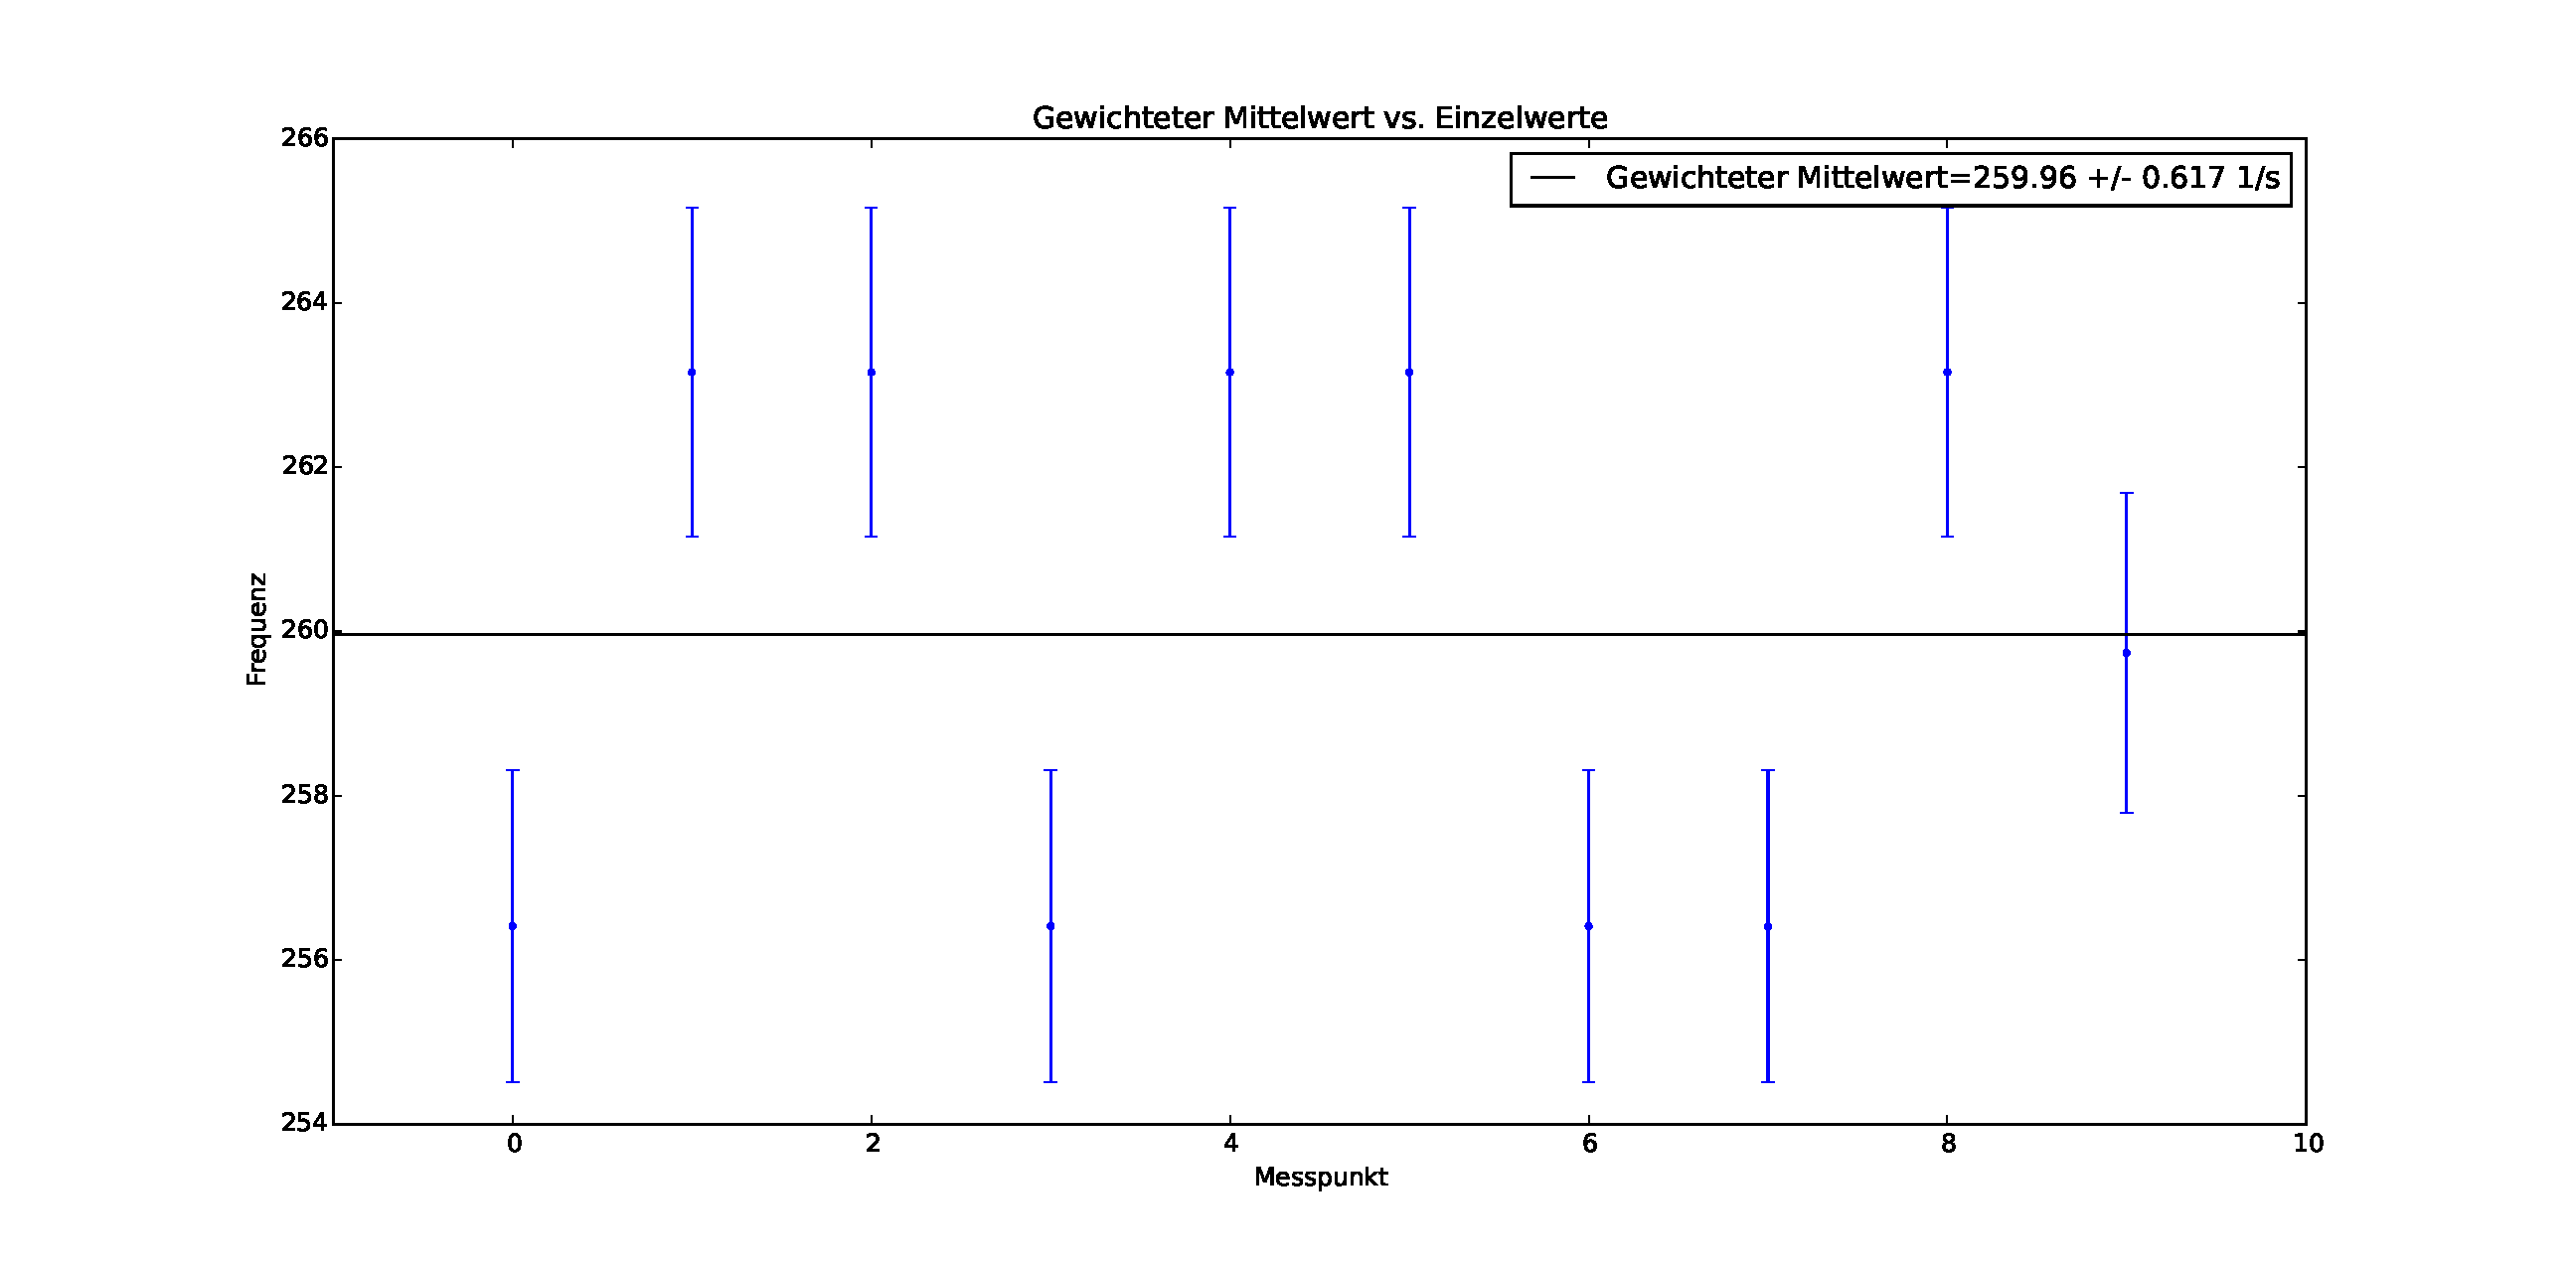
\includegraphics[scale=0.25]{Bilder/FrequenzGewichtet.eps}
\label{Frequenz_Oszi}
\end{figure}
\end{frame}

\begin{frame}
\begin{figure}[H]
\caption{Abklingkoeffizient}
\centering
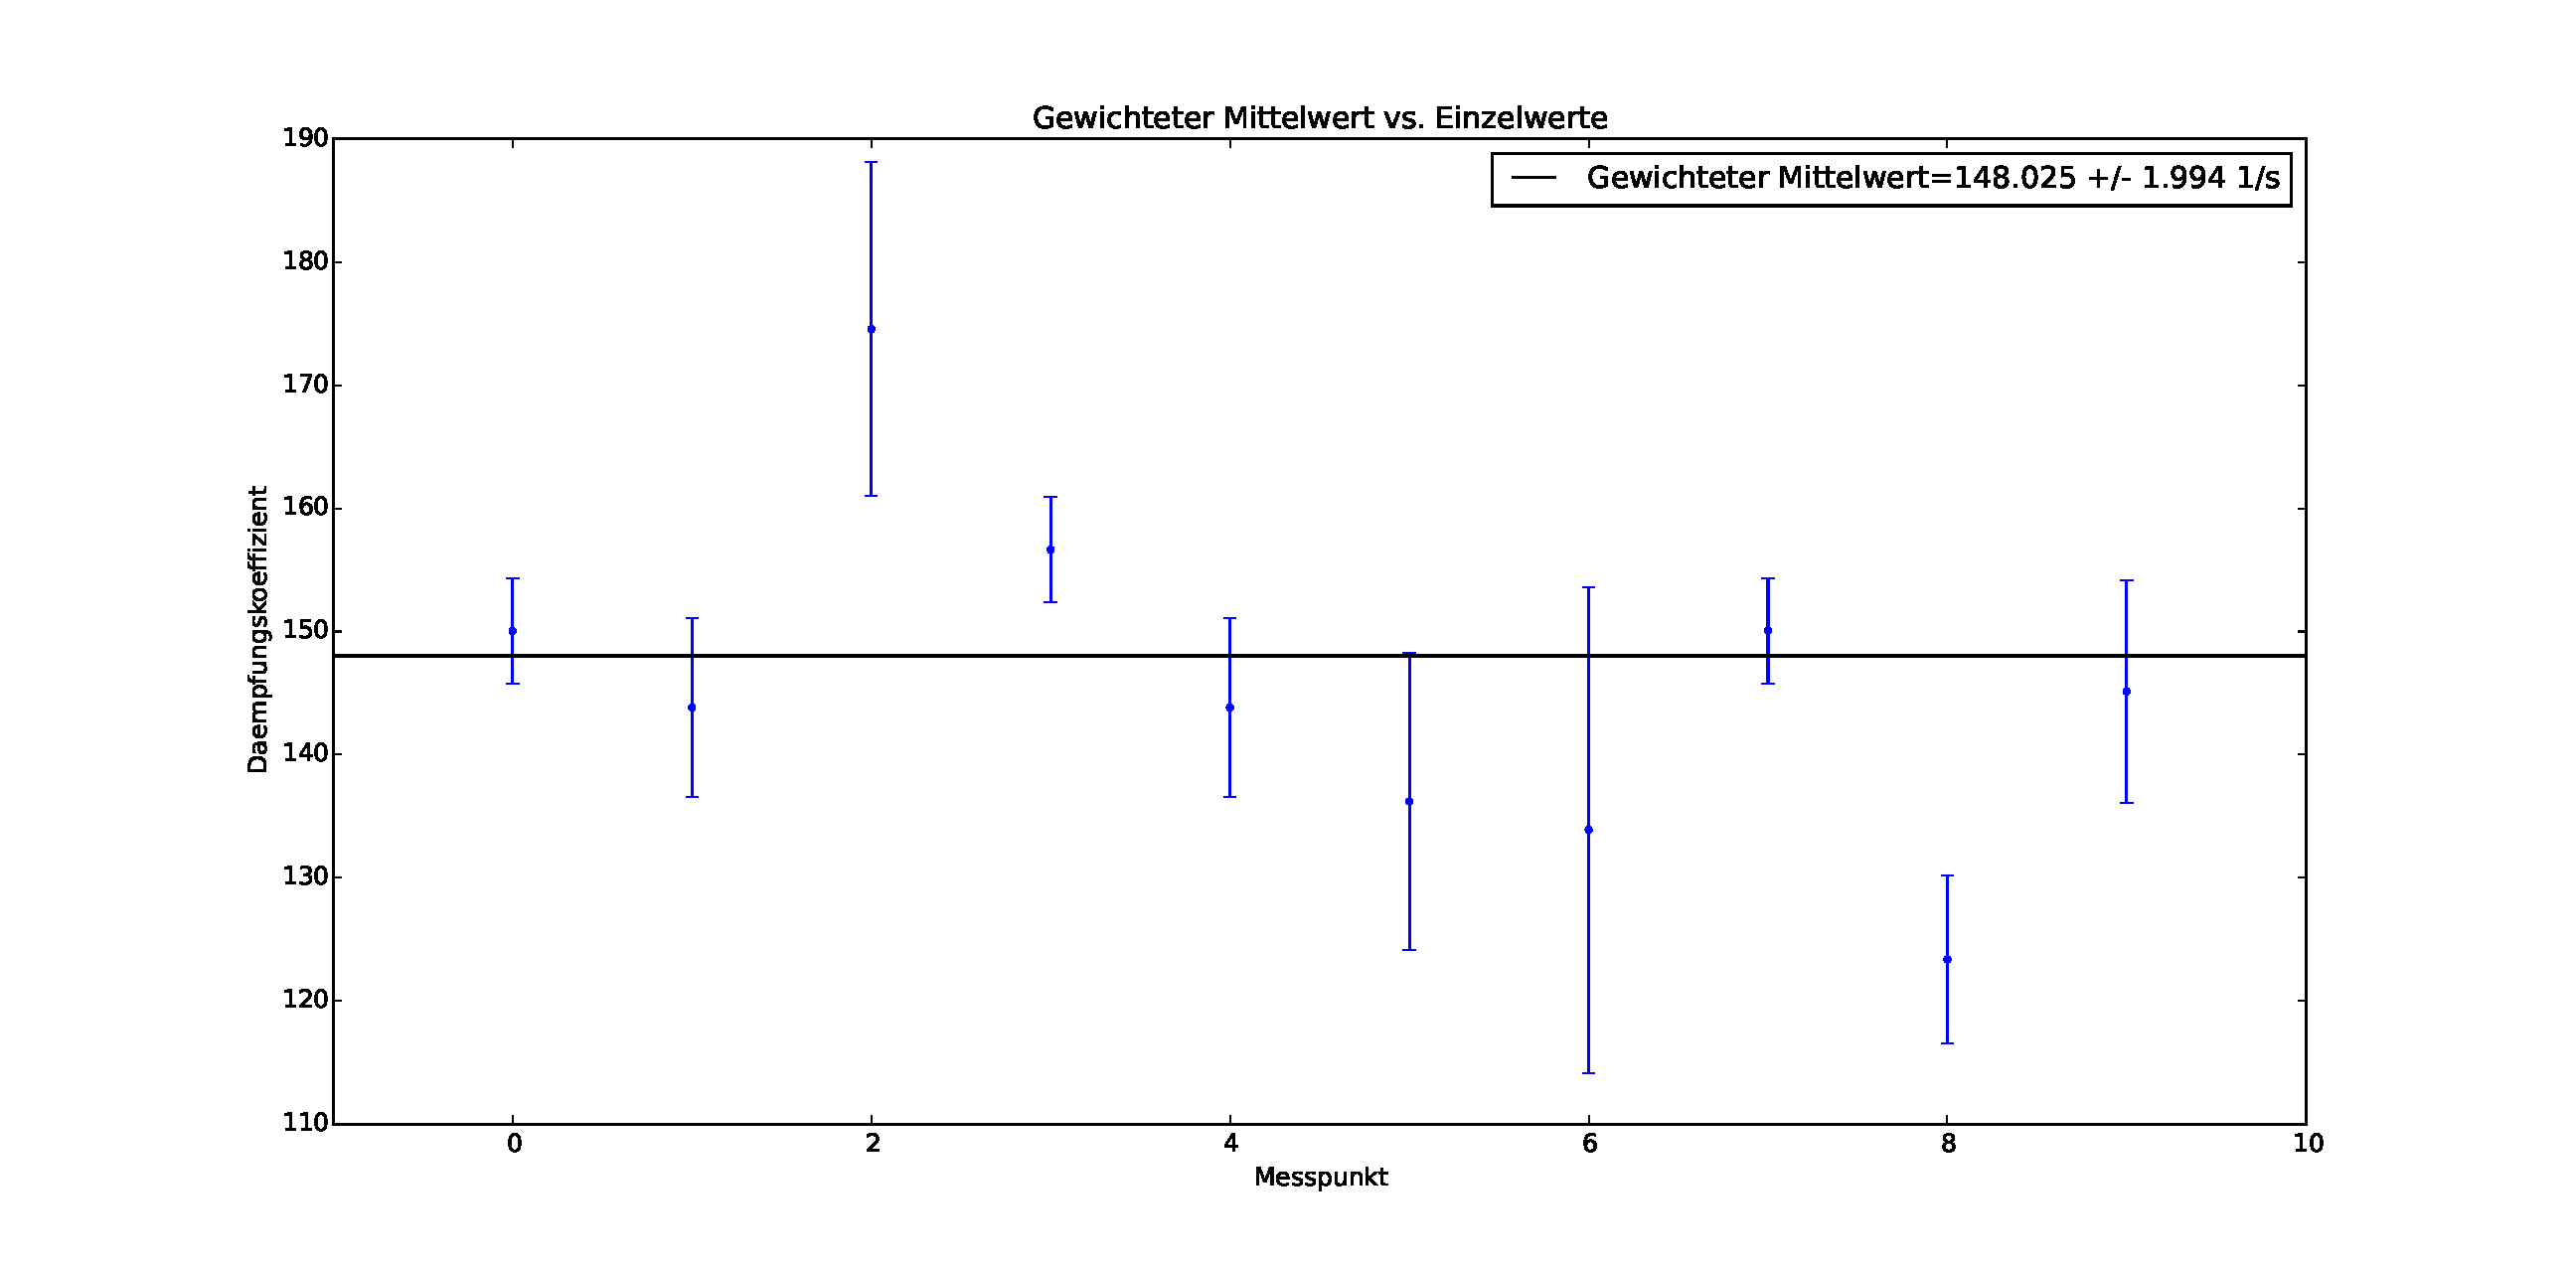
\includegraphics[scale=0.25]{Bilder/DaempfungGewichtet.eps}
\end{figure}
\end{frame}

\begin{frame}{Zusammenfassung der Analyse/ Fazit}
\begin{itemize}

\item Es fällt auf, dass $\delta$ größer ist als $\delta_{theo}$. Der Grund dafür ist, dass $\delta \sim R$ und wir bei R mit Sicherheit einen höheren Wert erwarten müssten, da zum Beispiel alle Bauteile einen Innenwiderstand aufweisen. 
\newline
\item Die jeweiligen Fehler auf die Mittelwerte liegen in einem realistischen Rahmen.
\end{itemize}
\end{frame}

\end{document}